\part{Premier pas vers SymPy}
\chapter{Premier pas vers SymPy}

Ce chapitre d’introduction présente la tournure d'esprit de la bibliothèque mathématique SymPy. Les 
autres chapitres de cette partie développent les notions de base de SymPy: effectuer des calculs 
numériques ou symboliques en analyse, opérer sur des vecteurs et des matrices, écrire des programmes, 
manipuler des listes de données, construire des graphiques, etc. Les parties suivantes de cet ouvrage 
approfondissent quelques branches des mathématiques dans lesquelles l'informatique fait preuve d'ne 
grande efficacité.

\section{La bibliothèque SymPy}

\subsection{Le cas de la bibliothèque SymPy}

Dans un cas plus simple l'exemple 1.1 se formule beaucoup plus dans un outil comme SymPy est une bibliothèque de calcul formel elle est aussi un environnement pour 
l’apprentissage de l'algèbre, l’analyse, géométrie, combinatoire, cryptographie, mécanique 
classique et quantique pour le lycée et l’université mais aussi un environnement de 
développement et de recherche. SymPy  écrit entièrement en Python un langage de 
programmation facile à apprendre et adapté à l’apprentissage,  elle fourni aux étudiant 
\textit{SymPyGamma} une application web   notamment des primitives générales de traitement des 
expressions algébriques (développement, factorisation, …), des aides à l’organisation des objets 
mathématiques intervenant dans la résolution d’un problème ainsi qu’une assistance à la preuve. Il 
permet au professeur de préparer et de suivre le travail de l’élève. Différentes maquettes ont été 
développées et testées auprès d’élèves. Dans la plus récente, nous nous sommes attachés à explorer une 
nouvelle forme d’activité algébrique. Alors que le calcul en papier crayon et les logiciels standards 
considèrent  les expressions de façon isolée, l’environnement que nous développons organise en réseau 
les différentes expressions intervenant dans la résolution d’un problème. L’ordinateur peut facilement 
mettre à jour ce réseau quand l’utilisateur modifie certains de ses éléments. Il devient ainsi possible, 
pour aborder un problème générique, d’explorer facilement des cas particuliers et de conduire une 
généralisation. Les relations entre expressions algébriques sont mieux mises en évidence du fait de leur 
invariance dans les modifications du réseau. De façon très concise, Casyopée peut être défini
\subsection{Travaillez avec SymPy}
\subsection{Installation de SymPy}

\subsection{isympy}
  \begin{python}
IPython console for SymPy 1.3 (Python 3.6.7-64-bit) (ground types: python)
These commands were executed:
>>> from __future__ import division
>>> from sympy import *
>>> x, y, z, t = symbols('x y z t')
>>> k, m, n = symbols('k m n', integer=True)
>>> f, g, h = symbols('f g h', cls=Function)
>>> init_printing()

Documentation can be found at http://docs.sympy.org/1.3/

  \end{python}
\subsection{SymPyGamma}
Est une interface onWeb marche avec un navigateur contient plusieurs catégorie liée de calcul, dynamique. L’Intérêt de cette outil qu'il est facilement partageable adapté pour l’enseignement et surtout l'auto-apprentissage

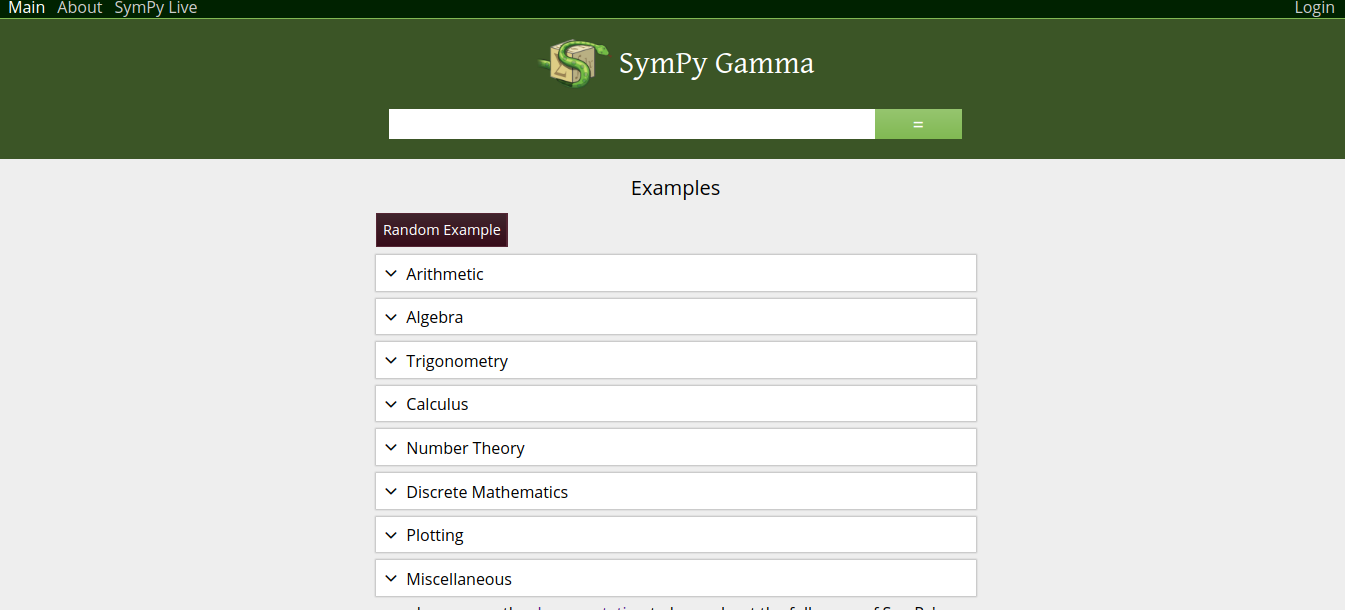
\includegraphics[scale=0.3]{../Pictures/sympyGammaMain.png} 

\subsection{SymPyLive}
SymPy Live est SymPy qui s'exécute sur Google App Engine. Ceci est juste un shell Python standard, avec les commandes suivantes exécutées par défaut
\section{SymPy comme calculatrice}
Contrairement à Sage[], Maple, Octave et les autres logiciel de calcul formel, SymPy, effectue des calculs directe numériques de deux manière différents en passant par la méthode, 
\subsection{Premier calculs}
Dans la suite du livre, nous présentons les calculs sous la forme suivante, qui
imite l’allure d’une session de SymPyLive à travers la ligne de commande isympy:
\begin{python}
In [1]: from sympy import *
In [2]: 1+1                                                                     
Out[2]: 2
\end{python}
\subsubsection{Variables Python}
Lorsque l’on veut conserver le résultat d’un calcul, on peut l’affecter à une
variable :

\subsubsection{Variables Symboliques}
Les objets mathématiques manipulés par SymPy sont symboliques ils sont représentés exactement loin de 
toute approximation numérique, SymPy permet une manipulation avec des expressions contenant
des variables, comme $x^{2} + zy^{3} + z^{2}$ ou encore $sin(x) - exp(x)$. Les variables symboliques
du mathématicien $x$, $y$, $z$ apparaissant dans ces expressions diffèrent, avec SymPy,
des variables du développeur $sin(2) = 0.9092974268256817$ que nous manipulons sous Python 
section précédente. SymPy diffère notablement, sur ce point, d’autres systèmes de calcul
formel comme Maple ou Maxima, Sage c'est inspiré de SymPy sur ce point.
\\

La documentation officiel présente la différence entre valeur numérique gérer par la bibliothèque
standard Python math à travers l'exemple de la racine carré $\sqrt{8}$ sans évaluation,
posons $x=8$

\begin{python}
In [1]: import math                                                             
In [2]: math.sqrt(x)                                                            
Out[2]: 2.8284271247461903
\end{python}
Les variables symboliques doivent \^etre explicitement déclarées avant d'\^etre employées

Dans cet exemple, la commande SR.var(’z’) « construit » et renvoie une variable symbolique dont le nom est z. Cette variable symbolique est un objet Sage comme un autre : elle n’est pas traitée différemment d’expressions plus complexes comme $sin(x) + 1$. Ensuite, cette variable symbolique est affectée à la variable « du programmeur » z, ce qui permet de s’en servir comme de n’importe quelle expression pour construire des expressions plus complexes.


\begin{python}
In [1]: from sympy import *
In [2]: x = symbols('x')                                                                     
In [3]: type(x)
Out[3]: sympy.core.symbol.Symbol
\end{python}

\begin{python}
In [4]: x+3                                                                     
Out[4]: x + 3
\end{python}

\subsection{Structure de données dans SymPy}
Le moteur symbolique de SymPy tire parti de l'orientation des objets (notamment l'héritage) pour créer une base de code facilement extensible. Toutes les classes dérivent des fonctionnalités, telles que la possibilité de se comparer à d'autres objets, à partir de méthodes de la super-classe Basic. Les objets pouvant faire l'objet d'opérations algébriques acquièrent cette capacité grâce à un ensemble de méthodes d'une classe appelée Expr. Ces objets Expr peuvent être conservés dans des objets conteneur (qui contiennent également la sous-classe Expr) Mul, Add et Pow; les objets conteneur sont instanciés à l'aide de l'opérateur Python, tel que la fonction de surcharge, qui permet au constructeur de la classe conteneur d'être appelé chaque fois que l'opérateur binaire approprié est utilisé (* pour Mul, + pour Ajouter et $**$ pour Pow).
De cette manière, des objets supplémentaires peuvent être ajoutés en créant simplement une sous-classe qui hérite des fonctionnalités de la classe Expr. Ces sous-classes bénéficient gratuitement de certaines fonctionnalités, telles que la possibilité de comparer, de multiplier, d’ajouter, etc. Voici comment SymPy crée un environnement modifiable, maintenable, et donc facile à étendre. Grâce à la possibilité d'hériter des propriétés de classes supérieures, la quantité de code nécessaire pour développer, par exemple, un système modélisant la mécanique quantique et la notation Dirac décroissant de manière significative.

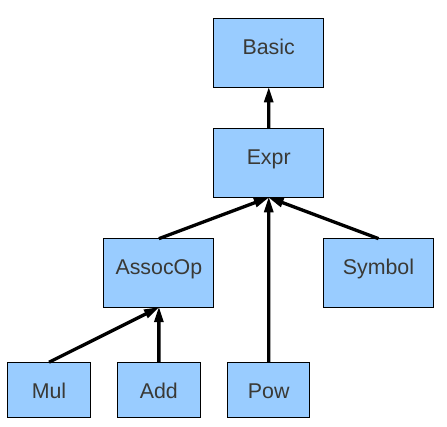
\includegraphics[scale=0.5]{../Pictures/sympyarch.png} 
\subsection{Variable et affection}\index{Variable et affection}

\begin{exercise}
Affectez les variables temps $t$ et distance $d$ par les valeurs 6.892 et 19.7. Calculez et affichez la valeur de la vitesse. Améliorez l'affichage en imposant un chiffre après le point décimal.
\end{exercise}

\begin{solution}
Pour, affectez des variables est les rendre symbolique comme c'est décrit dans le mémo ou il 
sera expliquer temps $t$ et distance $d$ par les valeurs 6.892 et 19.7. Calculez et affichez la 
valeur de la vitesse. Améliorez l'affichage en imposant un chiffre après le point décimal.
\end{solution}

\subsection{Substitution}
Une des choses les plus courantes que vous pourriez vouloir faire avec une expression mathématique est la substitution. La substitution remplace toutes les occurrences de quelque chose dans une expression par quelque chose d'autre. SymPy utilisant la méthode \textbf{subs}. Sym

\subsection{Contrôle du flux d’instructions}\index{Theorems!Single Line}
This is a theorem consisting of just one line.

\begin{exercise}
A set $\mathcal{D}(G)$ in dense in $L^2(G)$, $|\cdot|_0$. 
\end{exercise}
\begin{solution}
\end{solution}
%------------------------------------------------

\chapter{Analyse et Algèbre}\index{Analyse et Algèbre}
Ce chapitre présente à travers des exemples simples les fonctions de base utiles en analyse et en algèbre. Les 
lycéens et étudiants trouveront matière à  remplacer le crayon et le papier par le clavier et l'écran tout en 
relevant le même défi intellectuel de compréhension des mathématiques.Cet exposé des principales commandes de calcul 
avec Sage se veut accessible aux élèves de lycée.

\section{Expressions symboliques et simplification}\index{Expressions symboliques et simplification}
 \subsection{Expressions symboliques}
La bibliothèque SymPy permet d'effectuer toutes sortes de calculs d'analyse à partir d'expressions
symboliques combinant des nombres, des variables symboliques, les quatre opérations, et des fonctions usuelles comme 
sqrt, exp, log, sin, cos, etc. Une expression symbolique peut être représentée par un arbre comme ceux de la. Il est 
important de comprendre qu'une expression symbolique est une formule et non pas une valeur ou une fonction 
mathématique. Ainsi, SymPy ne reconnaît pas que les deux expressions suivantes sont égales
\subsection{Transformation d'expressions}\index{Transformation d'expressions}
\subsection{Fonctions mathématiques usuelles}\index{Fonctions mathématiques usuelles}
La plupart des fonctions mathématiques se retrouvent dans SymPy, en particulier les
fonctions trigonométriques, le logarithme et l'exponentiel : elles sont rassemblées
dans le tableau

\section{Équations}
Ceci est la documentation officielle du module solveset dans les solveurs. Il contient les questions fréquemment posées sur notre nouveau module pour résoudre des équations.
 \subsection{Résolution explicite}\index{Résolution explicite}
 \subsection{Équations sans solution explicite}\index{Équations sans solution explicite}
Dans la plupart des cas, dès que le système devient trop compliqué, il n’est pas possible de calculer une solution explicite
\section{In\'equations}\index{In\'equations}
\section{Analyse}\index{Analyse}
Dans cette section, nous présentons succinctement les fonctions couramment utiles en analyse réelle et complexe. 
Pour une utilisation avancée ou des compléments
 \subsection{Les Fonctions}\index{Fonctions}
Il sert également de constructeur pour les classes de fonctions non définies.

\begin{python}
from sympy import Function, Symbol
\end{python}

\begin{exercise}
Écrire une fonction cube qui retourne le cube de son argument
\end{exercise}

\begin{exercise}
Écrire une fonction $volumeSphere$ qui calcule le volume d’une sphère de rayon $r$ fourni
en argument et qui utilise la fonction cube .
Tester la fonction $volumeSphere$ par un appel dans le programme principal.
\end{exercise}

\begin{exercise}
Écrire une fonction maFonction qui retourne $f(x) = 2x^{3} + x - 5$
\end{exercise}

\begin{exercise}
Écrire une fonction tabuler avec quatre paramètres : $fonction$ , $borneInf$ , $borneSup$
et $nbPas$ . Cette procédure affiche les valeurs de $fonction$ , de $borneInf$ à $borneSup$ ,
tous les nbPas . Elle doit respecter $borneInf < borneSup$.
Tester cette fonction par un appel dans le programme principal après avoir saisi les
deux bornes dans une floatbox et le nombre de pas dans une integerbox (utilisez le
module easyguiB ).
\end{exercise}

\begin{exercise}
Écrire une fonction $volMasse$ Ellipsoide qui retourne le volume et la masse d'un ellipsoïde grâce à un tuple. Les paramètres sont les trois demi-axes et la masse volumique. On donnera à ces quatre paramètres des valeurs par défaut. \\
On donne: $v = \frac{3}{4} \pi abc$ \\
Tester cette fonction par des appels avec différents nombres d'arguments.
\end{exercise}

\begin{exercise}
Une fonction $f (x)$ est lin\'eaire et a une valeur de $29$ \`a $x = -2$ et $39$ à $x = 3$. Trouver sa valeur à $x = 5$.
\end{exercise}

\begin{exercise}
Pour l'ensemble $N$ de nombres naturels et une opération binaire $f: N x N \longrightarrow N$, on appelle un élément $z$ $\epsilon$ $N$ une identité pour $f$, si $f (a, z) = a = f (z, a)$, pour tout a $\epsilon$ $N$. Lesquelles des opérations binaires suivantes ont une identité?:
\begin{enumerate}
  \item $f (x, y) = x + y - 3$
  \item $f (x, y) = max(x, y)$
  \item $f (x, y) = x^{y}$
\end{enumerate}
\end{exercise}
\begin{solution}
le deuxième et le troisième 
\end{solution}
 \subsection{Sommes}
 \subsection{Limites}
Pour calculer une limite, on utilise la commande $\mathrm{limit}$. Soient à calculer les limites suivantes
%\begin{enumerate}
% \item $\frac{X}{Y}$
% \item $\frac{\sin(\frac{\pi}{2}-x)-\cot(x)}{1-\cos(\frac{\pi}{3}+x)$
%\end{enumerate}
 \subsection{Suites}
 Les fonctions précédentes permettent d’effectuer des études de suites. On donne un exemple d’étude de croissance comparée entre une suite exponentielle et une suite géométrique
 \subsection{Développements limités}
 SymPy peut calculer des développements de séries asymptotiques de fonctions autour d'un point. Pour calculer l'expansion de f (x) autour du point $x = x_{0}$ termes d'ordre xn, utilisez f(x).series(x, x0, n). x0 et $n$ peuvent être omis, auquel cas les valeurs par défaut x0 = 0 et $n = 6$ seront utilisées
 
 Pour calculer un développement limité d’ordre $n$ au sens fort $2$ en $x_{0}$, on dispose de la fonction $f(x).series(x==x0, n)$. Si l’on ne s’intéresse qu’à la partie régulière du développement limité à l’ordre n (au sens faible), on peut aussi utiliser la fonction taylor(f(x), x, x0, n)
 \begin{exercise}
 \end{exercise}
 \begin{exercise}
 \end{exercise}
 \begin{exercise}
 \end{exercise}
 \subsection{Séries}
  On peut utiliser les commandes précédentes pour effectuer des calculs sur les séries. Donnons quelques exemples.
 \subsection{Dérivation}
 La fonction derivative (qui a pour alias diff) permet de dériver une expression symbolique ou une fonction symbolique
 \subsection{Dérivées partielles}
 La commande diff permet également de calculer des dérivées n-ièmes ou des dérivées partielles.
 \subsection{Intégration}
 \section{Calcul matriciel}
  Dans cette section, on décrit les fonctions de base utiles en algèbre linéaire :opérations sur les vecteurs, puis sur les matrices. Pour plus de détails, on renvoie au chapitre 8 pour le calcul matriciel symbolique et au chapitre 13 pour le calcul matriciel numérique.
  \subsection{Résolution de systèmes linéaires}\index{Résolution de systèmes linéaires}
  \subsection{Calcul vectoriel}\index{Calcul vectoriel}
  Les fonctions de base utiles pour la manipulation des vecteurs sont résumées dans le tableau 2.5. On peut se servir de ces fonctions pour traiter l'exercice suivant.
  \subsection{Calcul matriciel} \index{Calcul matriciel}
  \subsection{Réduction d'une matrice carrée}\index{Réduction d'une matrice carrée}
 \chapter{Graphiques}
La visualisation de fonctions d'une ou deux variables, d'une série de données, facilite la perception de phénomènes mathématiques ou physiques et permet de conjecturer des résultat Équations sans solution explicitement efficacement. Dans ce chapitre, on illustre sur des exemples les capacités graphiques de SymPy.
 \section{Courbes en 2D}\index{Courbes en 2D}
 Une courbe plane peut être définie de plusieurs façons : comme graphe d'une fonction d'une variable, par un système d'équations paramétriques, par une équation en coordonnées polaires, ou par une équation implicite. Nous présentons
ces quatre cas, puis donnons quelques exemples de tracés de données.
 \subsection{Représentation graphique de fonctions}\index{Représentation graphique de fonctions}
 \subsection{Courbe paramétrée}\index{Courbe paramétrée}
 Les tracés de courbes paramétrées $(x = f(t), y=g(t))$ sont réalisés par la commande Curve\footnote{du module sympy.geometry(quand on le verra dans le chapitre)}$((f(t), g(t)), (t, a, b))$ ou $\left[a, b\right]$ est l'intervalle parcouru par le paramètre.
 \\
 Représentons par exemple la courbe paramétrée d'équations :
  
 \subsection{Courbe en coordonnées polaires}\index{Courbe en coordonnées gpolaires}
 \subsection{Courbe définie par une équation implicite}\index{Courbe définie par une équation implicite}
 Pour représenter une courbe donnée par une équation implicite, on utilise la fonction \textbf{plot\_implicit}
 $(f(x, y), (x, a, b), (y, c, d))$
 \subsection{Tracé de données}\index{Tracé de données}
 \subsection{Tracé de solution d'équation différentielle}\index{Tracé de solution d'équation différentielle}
 
 \subsection{Développée d'une courbe}\index{Développée d'une courbe}
 \section{Courbes en 3D}   
